\documentclass[12pt]{article}
\usepackage{amsmath, booktabs, caption, scrextend, graphicx, listings}
\graphicspath{ {.} }

\title{First Assignment}
\author{Mariano D'Angelo}
\date{$1^{st}$ March 2022}

\begin{document}

\maketitle


\section*{Task 1}
Calculate GCD(a, b) and find Bezout's identity for a=2022, b=752. \\\\
\begin{tabular}{ | c | c | c | } \hline
    \textbf{rem} & \textbf{val} & \textbf{expr} \\ \hline
    $r_0$ & 2022 & a \\
    $r_1$ & 752 & b \\
    $r_2$ = $r_0$ mod $r_1$ & 518 & a - 2b \\
    $r_3$ = $r_1$ mod $r_2$ & 234 & b - (a - 2b) = 3b - a \\
    $r_4$ = $r_2$ mod $r_3$ & 50 & (a - 2b) - 2(3b - a) = 3a - 8b \\
    $r_5$ = $r_3$ mod $r_4$ & 34 & (3b - a) - 4(3a - 8b) = 35b - 13a \\
    $r_6$ = $r_4$ mod $r_5$ & 16 & (3a - 8b) - (35b - 13a) = 16a - 43b \\
    $r_7$ = $r_5$ mod $r_6$ & 2 & (35b - 13a) - 2(16a - 43b) = 121b - 45a \\ \hline
    $r_8$ = $r_6$ mod $r_7$ & 0 & \\ \hline
\end{tabular}

\noindent \newline \newline The gcd of 2022 and 752 is \textbf{2}. \newline
From the final line of the table we can see that Bezout's identity is fulfilled
with \textbf{-45} for x and \textbf{121} for y.\newline
This can be checked with: $(2022 \cdot (-45)) + (752 \cdot 121)$ = 2

\pagebreak


\section*{Task 2} 

Solve the following congruences: \\

\noindent 1) x + 17 = 23 (mod 37) \textbar{} -17
\begin{addmargin}[1.22em]{0em}
x + 17 - 17 = 23 - 17 (mod 37) \\
x = 6 (mod 37) \\
x = \textbf{6} \\
\end{addmargin}

\noindent2) x + 42 = 19 (mod 51) \textbar{} -42
\begin{addmargin}[1.22em]{0em}
x + 42 - 42 = 19 - 42 (mod 51) \\
x = -23 (mod 51) \\
x = -23 + 51 (mod 51) \\   
x = 28 (mod 51) \\
x = \textbf{28}
\end{addmargin}


\section*{Task 3} 

Solve the following congruences: \\

\noindent 1) $23^{37}$ mod 40 = 
\begin{addmargin}[1.22em]{0em}
$23 \cdot 23^{36}$ mod 40 = \\
$23 \cdot 23^{12\cdot3}$ mod 40 = \\
$23 \cdot 23^{4\cdot3\cdot3}$ mod 40 = \\
$23 \cdot 23^{2\cdot2\cdot3\cdot3}$ mod 40 = \\
$23 \cdot 529^{2\cdot3\cdot3}$ mod 40 = \\
$23 \cdot (529^{2\cdot3\cdot3}$ mod 40) mod 40 = \\
$23 \cdot 9^{2\cdot3\cdot3}$ mod 40 = \\
$23 \cdot 81^9$ mod 40 = \\
$23 \cdot 1^9$ mod 40 = 
\textbf{23}
\end{addmargin}

\pagebreak

\noindent 2) $(-133)^{100}$ mod 10 = 
\begin{addmargin}[1.22em]{0em}
(-133 mod 10)$^{100}$ mod 10 = \\
$7^{100}$ mod 10 = \\
$7^{4 \cdot 25}$ mod 10 = \\
$2401^{25}$ mod 10 = \\
$1^{25}$ mod 10 = 
\textbf{1}
\end{addmargin}

\section*{Task 4}

Consider the following sequence of operations: 
\\

\noindent $Plaintext \rightarrow S_1 \rightarrow P_1 \rightarrow S_2 \rightarrow P_2 \rightarrow Ciphertext$
\\

\noindent Plaintext is \textbf{MOTIVATION}. $S_1$ is a shift cipher with key $k_{S_1}$ = 17.
$S_2$ is a shift cipher with the key $k_{S_2}$ = 8. $P_1$ is a permutation cipher 
with a key \\ $k_{P_1}$ = (5,1,3,2,4). $P_2$ is a permutation cipher with a key 
$k_{P_2}$ = (3,4,5,1,2). \\\\ \textbf{The task:} what is the ciphertext? \\

\noindent This task was solved both with code and manually. The shift into Caesar cipher
was made by a Python script I wrote in Appendix A. The code has one global variable
called alphabet that stores two entire English alphabets. This was made in order to
avoid the string index out of range in case the shift makes a number greater than 26, in that
case the alphabet restart from a, but not as 0 but 26. The main function is called tocaesar,
which takes a plaintext and the desired shift as input and encrypts the plaintext.
In order to encrypt every single letter I ran a loop for each in the text, then I 
found the index of the every inspected letter and assigned it to a temporary variable
called position. Once we get the position we need to calculate the new shifted one
so I just summed the old position with the input shift. Knowing the
new shifted position of the letter, I appended the corresponding 
alphabet letter with the index of
the new position to an initially empty string called result. 
The transposition part was made by hand. \\

\noindent After running the script for the first time giving input of MOTIVATION and
17 we get the first ciphertext \textbf{dfkzmrkzfe}. \\

\noindent Now with the key (5, 1, 3, 2, 4) we need to transpose the current text. \\

\noindent 1  2  3  4  5  1  2  3  4  5 \\
d  f  k  z  m  r  k  z  f  e \\

\noindent 5  1  3  2  4  5  1  3  2  4 \\
m  d  k  f  z  e  r  z  k  f \\

\noindent After running the script again giving input of mdkfzerzkf and 8 we get the
third ciphertext \textbf{ulsnhmzhsn}. \\

\noindent Finally we can run the final transposition and get the final result using
the following key (3,4,5,1,2). \\

\noindent 1  2  3  4  5  1  2  3  4  5 \\
u  l  s  n  h  m  z  h  s  n \\ 

\noindent 3  4  5  1  2  3  4  5  1  2 \\
s  n  h  u  l  h  s  n  m  z \\

\noindent The final ciphertext is: \textbf{snhulhsnmz}.


\section*{Task 5}

Assume that the Affine cipher is implemented $Z_{89}$, not in $Z_{26}$.
\newline

\noindent
\textbf{1. Write down encryption and decryption functions for this modification of Affine cipher.}\newline

\noindent a, b - together form the key k(a, b) \\
m - plaintext message \\
c - ciphertext \\\\
\noindent The encryption key is: $E_m$ = am + b mod 89 \\
The decryption key is: $D_c$ = $a^{-1} \cdot (c - b)$ mod 89 \pagebreak 

\noindent \textbf{2. What is the number of possible keys?}
\newline
\noindent
\\The number of possible keys is: $89 \cdot \Theta(89)$ or $89 \cdot 88$. 88 is 
what we get from the Euler's function, following the property: $\Theta(p) = p - 1$, 
where p represents a prime number. This means that there is a total of 7832 possible
keys.
\newline

\noindent \textbf{3. Suppose that modulus p = 89 is public. Malicious Eve intercepts 
two ciphertexts encrypted with the same key sent from Alice to Bob $c_1$ = 1 and
$c_2$ = 69. Assume that Eve also managed to find out that the corresponding 
plaintexts are $m_1$ = 10 and $m_2$ = 7. Find out the encryption key and use it 
to encrypt message $m_3$ = 13.}
\newline

\noindent Firstly, we write down the following system of equations:
$$\begin{cases}
    69 = 7a + b \text{mod 89} \\
    1 = 10a + b \text{mod 89} 
\end{cases}$$

Now we can solve it and find the key k(a, b). 
$$\begin{cases}
    69 = 7a + b \text{mod 89} \hspace{0.1cm} | \cdot (-1) \\
    1 = 10a + b \text{mod 89} 
\end{cases}$$

$$\begin{cases}
    -69 = -7a - b \text{mod 89} \\
    1 = 10a + b \text{mod 89} 
\end{cases}$$

\noindent \\After this we get: \\

\noindent -69 + 1 = -7a + 10a + 0 mod 89 \\
-68 = 3a mod 89 \\
(-68 mod 89) = 3a mod 89 \\
21 = 3a mod 89 \textbar{} : 3\\
7 = a mod 89 \\
a = 7 mod 89 \\
a = 7 \\

\noindent Now that we have a we can find b by just replacing a's value into one of the equations in the system. \\

\noindent $69 = 7 \cdot 7$ + b mod 89 \\
69 = 49 + b mod 89 \\
69 - 49 = b mod 89 \\
20 = b mod 89 \\
b = 20 mod 89 \\
b = 20 \\

\noindent a and b form the encryption key \textbf{k(7, 20)}.
Knowing that $m_3$ = 13 we can insert it into the Affine encryption function
$E_m$ = am + b mod 89, knowing that a = 7 and b = 20. \\

\noindent The ciphertext we get is: \\

\noindent $7 \cdot 13$ + 20 mod 89 = \\
91 + 20 mod 89 = \\
111 mod 89 = 22 \\

\noindent Ciphertext $c_3$ is \textbf{22}.


\section*{Task 6}

Let the message be \\

\noindent \textit{"The most beautiful things in the world cannot be seen or touched, 
they are felt with the heart."} | Antoine de Saint-Exupery, The Little Prince \\

\noindent Make frequency table for that message and compute index of coincidence. \\

\noindent  In order to calculate the index of coincidence I wrote a small C program to do 
the trick. In main I declared three variables called alphabet, an array that contains all of 
the letters from the english alphabet, counter, an array of 26 0's, and txt that contains
the quote from Exupery. After their declaration a function called findIC is called that 
takes as input these three variables. The function loops through the text and for every letter stops,
compares the letter with the ones in the alphabet's array (this is done by the internal loop) and if there 
is a match the letter's respective counter (each letter has its own counter) increases by one. 
Also the length of the text is increased by one (I had to do it
manually in order to avoid counting spaces) and  finally the inner loop breaks. The outer loop only
ends when the txt pointer is pointing to the array's terminating 0. Once we have 
the length of the text and the counters for each of the letters I computed the index 
of coincidence with its respective formula. To compute the index of coincidence I ran a loop 
26 times, one time for each of the letter. In the end I return the IC as a double value and
print it. \\

\noindent The frequency table that we get is:  \\

\noindent 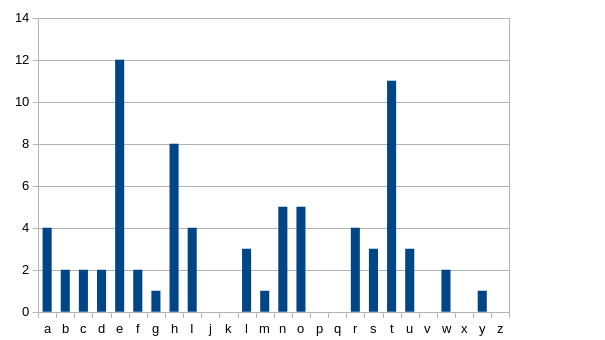
\includegraphics[scale=0.5]{frequency_table} \\

\noindent The index of coincidence is: \textbf{0.0724324}


\section*{APPENDIX A - task 4 program}

\begin{lstlisting}

alphabet = ['a', 'b', 'c', 'd', 'e', 'f', 'g', 'h', 'i', 'j', 'k', 'l', 'm', 
    'n', 'o', 'p', 'q', 'r', 's', 't', 'u', 'v', 'w', 'x', 'y', 'z']

alphabet += ['a', 'b', 'c', 'd', 'e', 'f', 'g', 'h', 'i', 'j', 'k', 'l', 'm', 
    'n', 'o', 'p', 'q', 'r', 's', 't', 'u', 'v', 'w', 'x', 'y', 'z']


def tocaesar(text, shift):
    result = ""
    for letter in text:
        position = alphabet.index(letter)
        newPosition = position + shift 
        result += alphabet[newPosition]
    return result


text = input("Type in the desired text: ")
shift = int(input("Type in the shift: "))
print(tocaesar(text, shift))

\end{lstlisting}

\section*{APPENDIX B - task 6 program}

\begin{lstlisting}

#include <stdio.h>


double findIC(char* txt, char* alphabet, int* counters) {
    int txtLength = 0;
    for (int i = 0; *(txt + i); i++) {
        for (int j = 0;  j < 26; j++) {
            if (*(txt + i) == *(alphabet + j)) {
                *(counters + j) += 1;
                txtLength++;
                break;
            }
        }
    }
    double ic = 0;
    for (int i = 0; i < 26; i++) {
        ic += ((double)counters[i] / txtLength) * 
            ((double)(counters[i] - 1) / ( txtLength - 1)); 
    }
    return ic;
}


int main() {
    char alphabet[] = "abcdefghijklmnopqrstuvwxyz";
    int counters[26] = {0};
    char txt[] = "The most beautiful things in the world cannot be" 
        "seen or touched, they are felt with the heart.";
    double ic = findIC(txt, alphabet, counters);
    printf("The index of coincidence for the text is: %lg\n", ic);
    return 0;
}

\end{lstlisting}
\end{document}
